%%%%%%%%%%%%%%%%%%%%%%%%%%%%%%%%%%%%%%%%%%%%%
\section{Code validation}
\label{Sec:Validation}
%%%%%%%%%%%%%%%%%%%%%%%%%%%%%%%%%%%%%%%%%%%%%

In this section we validate the numerical methods described in the previous section. We start with the mixing of a gas whose self-gravity is neglected, for which the exact solution is known. Next, we show that the functions $h_n(t)$ need to be computed with the action-angle variables which belong to the total potential, and we quantify the departure of the discretized steady states from stationarity as well as the time span over which the quiet start of section~\ref{SubSec:QuietStart} is reliable. Then, we analyze the dependency of the response of the gas on the time step and on the amplitude of the perturbation, and we compare it with the solution of the linearized equations. Finally, we test the linearized solver and the computation of the gain $\lambda(\omega)$ against each other.


\subsection{Mixing in the absence of self-gravity}
\label{SubSec:ValFree}

When the last term in the second equation in~(\ref{Eq:EOM}) is omitted, the computational particles move independently from each other in the external potential, and the functions $h_n(t)$ are given by Eq.~(\ref{Eq:hnFree}). This provides a test for the time integration, for the representation of the DF by the lattice~(\ref{Eq:Lattice}) and for the computation of the observables. We consider the reduced model with $L_0 = 2$ in the isochrone potential and the initial DF
\begin{equation}
\mathcal{F}_0(0,Q,J) = \alpha\exp\left[ -\frac{\sin^2(Q/2)}{\sigma_Q^2} \right] J^2\exp\left( -\frac{J^2}{\sigma_J^2} \right),\qquad
\sigma_Q = \sigma_J = 0.1,
\label{Eq:Pulse}
\end{equation}
which describes a gas cloud whose particles are concentrated near the pericenters of their orbits (see Fig.~\ref{Fig:Pulse}), and we choose the weight function $B(J) = J^2\exp(-J^2/\sigma_J^2)$, that is, Eq.~(\ref{Eq:BDef}) with $J_1 = 0$ and $\sigma_1 = \sigma_J$.

The dependency of the DF~(\ref{Eq:Pulse}) on the angle variable has been chosen such that it is smooth and $2\pi$-periodic and such that its Fourier coefficients~(\ref{Eq:FourierF}) are known explicitly. In fact, the identity $\sin^2(Q/2) = (1 - \cos Q)/2$ yields
\begin{equation}
\exp\left[ -\frac{\sin^2(Q/2)}{\sigma_Q^2} \right] = e^{-z} e^{z\cos Q}
 = e^{-z}\sum\limits_{n\in\Integer} I_n(z) e^{inQ},\qquad
z := \frac{1}{2\sigma_Q^2},
\label{Eq:BesselExpansion}
\end{equation}
where $I_n$ denotes the modified Bessel function of the first kind of order $n$, which satisfies $I_{-n} = I_n$. The second equality in Eq.~(\ref{Eq:BesselExpansion}) is the generating function of these functions, see Eq.~(10.35.2) in Ref.~\cite{DLMF}; equivalently, $I_n(z)$ is the $n$-th Fourier coefficient of the function $e^{z\cos Q}$ (Eq.~(10.32.3) in Ref.~\cite{DLMF}). Consequently, the Fourier coefficients of the DF~(\ref{Eq:Pulse}) with respect to the angle variable are
\begin{equation}
\hat{F}_n(J) = \alpha\, e^{-z} I_n(z)\, J^2\exp\left( -\frac{J^2}{\sigma_J^2} \right).
\label{Eq:PulseFourier}
\end{equation}
For $\sigma_Q = 0.1$ one has $z = 50$, and in this case $I_n(z)/I_0(z)$ differs from $e^{-n^2/(2z)}$ by less than one percent for $|n|\leq 16$. Hence, the narrower the pulse is in the angle variable, the more harmonics it contains: here the amplitudes of those with $|n|\leq 2\sqrt{z}\approx 14$ are larger than $e^{-2}\approx 0.14$ times the one of the harmonic $n = 0$. It follows from Eqs.~(\ref{Eq:hnFree},\ref{Eq:PulseFourier}) that $|h_n(0)|/h_0 = I_n(z)/I_0(z)$, which is equal to $0.990$, $0.960$, $0.913$ and $0.851$ for $n = 1,2,3,4$, and that $h_n(t)$ is given by an integral over $J$, which we compute with the trapezoidal rule on $2\times 10^5$ subintervals of $0\leq J\leq 6\sigma_J$. The computational particles are placed on a lattice of the form~(\ref{Eq:Lattice}), consisting of $N_J$ rows which cover the interval $0 < J < 6\sigma_J$ and of $N_Q$ points per row, their masses are proportional to the values of the DF~(\ref{Eq:Pulse}) at the lattice points, and their radii and momenta are obtained from the explicit action-angle map of the isochrone potential.

\begin{figure}[htp]
\centerline{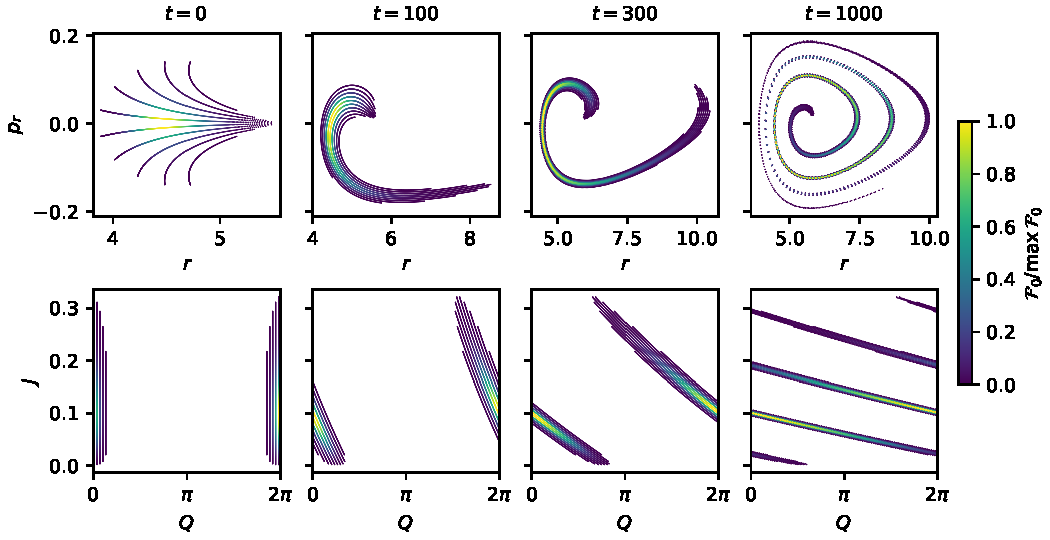
\includegraphics[width=0.85\textwidth]{figuras/validacion_pulso.pdf}}
\caption{Mixing of the initial datum~(\ref{Eq:Pulse}) in the isochrone potential when self-gravity is neglected. Shown are the computational particles in the $(r,p_r)$-plane (upper panels) and in the plane of the action-angle variables (lower panels) at four different times, for a lattice with $N_J\times N_Q = 800\times 64$ points. The color indicates the mass of each particle relative to the largest one, and only particles whose mass exceeds $10^{-3}$ of the latter are shown.}
\label{Fig:Pulse}
\end{figure}

\begin{table}[htp]
\begin{center}
\begin{tabular}{rrl|cccc}
\hline\hline
$N_J$ & $N_Q$ & $\Delta t$ & $e_1$ & $e_2$ & $e_3$ & $e_4$ \\
\hline
$50$ & $64$ & $0.1$ & $4.1\times 10^{-6}$ & $1.6\times 10^{-4}$ & $0.15$ & $0.72$ \\
$100$ & $64$ & $0.1$ & $3.3\times 10^{-8}$ & $1.2\times 10^{-7}$ & $5.1\times 10^{-7}$ & $3.9\times 10^{-6}$ \\
$200$ & $64$ & $0.1$ & $5.3\times 10^{-9}$ & $5.4\times 10^{-9}$ & $5.9\times 10^{-9}$ & $5.5\times 10^{-9}$ \\
$400$ & $64$ & $0.1$ & $5.3\times 10^{-9}$ & $5.5\times 10^{-9}$ & $6.0\times 10^{-9}$ & $5.5\times 10^{-9}$ \\
\hline
$400$ & $16$ & $0.1$ & $9.2\times 10^{-3}$ & $3.7\times 10^{-2}$ & $8.2\times 10^{-2}$ & $0.14$ \\
$400$ & $32$ & $0.1$ & $1.7\times 10^{-5}$ & $7.3\times 10^{-5}$ & $1.8\times 10^{-4}$ & $3.7\times 10^{-4}$ \\
\hline
$400$ & $64$ & $0.2$ & $8.6\times 10^{-8}$ & $8.8\times 10^{-8}$ & $9.6\times 10^{-8}$ & $8.8\times 10^{-8}$ \\
$400$ & $64$ & $0.05$ & $3.3\times 10^{-10}$ & $3.4\times 10^{-10}$ & $3.7\times 10^{-10}$ & $3.4\times 10^{-10}$ \\
$400$ & $64$ & $0.025$ & $2.1\times 10^{-11}$ & $2.0\times 10^{-11}$ & $2.2\times 10^{-11}$ & $2.7\times 10^{-11}$ \\
$400$ & $64$ & exact & $6.6\times 10^{-12}$ & $1.3\times 10^{-11}$ & $2.0\times 10^{-11}$ & $2.7\times 10^{-11}$ \\
\hline\hline
\end{tabular}
\end{center}
\caption{Error $e_n$ defined in Eq.~(\ref{Eq:FreeError}) for the mixing of the initial datum~(\ref{Eq:Pulse}) in the absence of self-gravity, for different lattices and time steps. In the last row the Yoshida integrator is replaced with the exact advance of the angle variables.}
\label{Tab:FreeMixing}
\end{table}

Table~\ref{Tab:FreeMixing} shows the error
\begin{equation}
e_n := \frac{1}{h_0}\max\limits_{0\leq t\leq 2000} \left| h_n(t) - h_n^{exact}(t) \right|
\label{Eq:FreeError}
\end{equation}
for different lattices and time steps. For $N_J\times N_Q = 400\times 64$ and $\Delta t = 0.1$ it does not exceed $6\times 10^{-9}$ for $n\leq 4$. In this case the error is dominated by the time integration. In fact, when the Yoshida integrator is replaced with the exact advance $Q_j\mapsto Q_j + \Omega(J_j)\Delta t$ of the angle variables of the particles, the error drops to less than $3\times 10^{-11}$, and the difference with respect to this solution decreases by the factors $16.0$, $16.0$ and $15.4$ each time $\Delta t$ is halved between $0.2$ and $0.025$ (for $n = 1$), as expected for a fourth-order method.

The remaining rows of Table~\ref{Tab:FreeMixing} show the effect of the lattice. Since the sum~(\ref{Eq:hnPIC}) is a midpoint rule for an integral whose integrand is smooth and, with respect to $Q$, periodic, the error decreases rapidly when $N_J$ or $N_Q$ increase, until it reaches the one of the time integration.

With respect to the angle variable the error of the lattice can be computed explicitly. On a lattice with $N_Q$ points per row the harmonics $n + mN_Q$, $m\in\Integer$, cannot be distinguished from the harmonic $n$, such that the sum over the points $Q_b$ yields $\sum_m (-1)^m\hat{F}_{n+mN_Q}$ instead of $\hat{F}_n$, where the signs are due to the fact that the $Q_b$ are the midpoints of the subintervals. Since the transport does not mix different harmonics, this factor is independent of time. Taking into account that the masses of the computational particles are normalized such that their sum is equal to $M_{gas}$, Eq.~(\ref{Eq:PulseFourier}) gives
\begin{equation}
e_n = \left| \frac{\sum_m (-1)^m I_{n+mN_Q}(z)}{\sum_m (-1)^m I_{mN_Q}(z)} - \frac{I_n(z)}{I_0(z)} \right| ,
\label{Eq:Aliasing}
\end{equation}
where the sums extend over all $m\in\Integer$. This expression reproduces the values in the rows with $N_Q = 16$ and $N_Q = 32$ of Table~\ref{Tab:FreeMixing} to nine significant digits, and for $N_Q = 64$ it is smaller than $5\times 10^{-15}$. Hence, the number of points per row has to be a few times larger than the number $2\sqrt{z}$ of harmonics contained in the DF.

With respect to the action variable the situation is different, since for a given lattice the sum is only reliable over a finite time span. The reason is that the phases $n\Omega(J_a)t$ of two neighboring rows differ by $n|\Omega'(J)|\Delta J\, t$, with $\Delta J$ the spacing between the rows. When this difference reaches $2\pi$ the rows are in phase again, such that $h_n$ exhibits a spurious recurrence~\cite{BirdsallLangdon-Book} at the time
\begin{equation}
t_{rec} = \frac{2\pi}{n|\Omega'(J)|\Delta J}.
\label{Eq:Recurrence}
\end{equation}
In the present example, $\Delta J = 0.6/N_J$ and $|\Omega'(J)|\leq 3/c(L_0)^4\approx 0.088$, which gives $t_{rec}\approx 120\, N_J/n$. For $N_J = 50$ this is $1980$ and $1480$ for $n = 3$ and $n = 4$, respectively, which explains the large values of $e_3$ and $e_4$ in the first row of the table. For the lattices which are used in the following subsections the recurrence time for $n = 1$ exceeds the duration of the simulations: it is $4.7\times 10^4$ for the one of section~\ref{SubSec:ValAA} and at least $1.3\times 10^4$ for those of sections~\ref{SubSec:ValStationarity} and~\ref{SubSec:ValResponse}.

\begin{figure}[htp]
\centerline{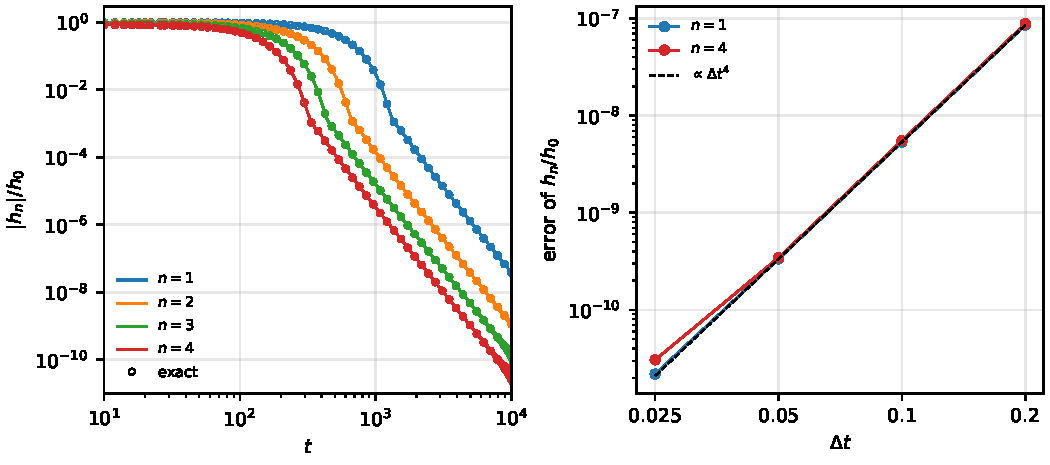
\includegraphics[width=0.85\textwidth]{figuras/validacion_libre.pdf}}
\caption{Left panel: the functions $|h_n(t)|/h_0$, $n = 1,2,3,4$, for the mixing of the initial datum~(\ref{Eq:Pulse}) in the absence of self-gravity, obtained from the PIC code with $N_J\times N_Q = 800\times 64$ and $\Delta t = 0.1$ (solid lines) and from the exact solution~(\ref{Eq:hnFree}) (circles). Right panel: error of the time integration, measured through the difference with the solution in which the angle variables are advanced exactly, as a function of the time step. The dashed line is proportional to $\Delta t^4$.}
\label{Fig:FreeMixing}
\end{figure}

Figure~\ref{Fig:FreeMixing} shows the result of a simulation with $N_J\times N_Q = 800\times 64$ and $\Delta t = 0.1$ which extends to $t = 10^4$. During this time $|h_1|$ and $|h_4|$ decay by seven and ten orders of magnitude, respectively, and the numerical solution reproduces the exact one over the whole range: for $n\leq 4$ the difference does not exceed $6\times 10^{-9} h_0$ at any time, and it is smaller than $2\times 10^{-10} h_0$ for $t\geq 5000$. At late times $|h_n(t)|$ is proportional to $t^{-5}$ (a fit over $5000\leq t\leq 10^4$ gives the exponents $-5.03$ and $-5.01$ for $n = 1$ and $n = 2$). This is the analogue of the algebraic tail~(\ref{Eq:Tail}) for the endpoint $J = 0$ of the support, at which the function $\hat{F}_n B$ vanishes like $J^4$. In the same simulation $h_0$, which is constant for the exact solution, varies by $1.1\times 10^{-9}$, and the total energy by $7\times 10^{-11}$, in relative terms.

For the code with a distribution of angular momenta we have performed the analogous test with the DF~(\ref{Eq:Pulse}) multiplied by the factor $\exp[-(L - L_0)^2/\sigma_L^2]$ with $\sigma_L = 0.2$, restricted to the interval $1.6\leq L\leq 2.4$, on a lattice with $N_J\times N_Q\times N_L = 200\times 40\times 16$ points and with $\Delta t = 0.025$ up to $t = 200$. The difference with respect to the exact advance of the same lattice points is $1.3\times 10^{-11} h_0$ for $n = 1$ and $2.6\times 10^{-11} h_0$ for $n = 4$. In this case the error is dominated by the quadrature with respect to $L$, whose integrand does not vanish at the boundaries of the interval: it is $2.0\times 10^{-4} h_0$ for $N_L = 16$ and decreases by a factor of four each time $N_L$ is doubled, down to $3.3\times 10^{-6} h_0$ for $N_L = 128$. \EJ{These numbers are taken from the notes of the code with a distribution of $L$; the test should be repeated with the parameters of this subsection.}


\subsection{Action-angle variables of the total potential}
\label{SubSec:ValAA}

As emphasized in section~\ref{SubSec:Observables}, the functions $h_n(t)$ with $n\neq 0$ measure the departure of the gas configuration from a steady state only if they are computed with the action-angle variables which belong to the total potential. To illustrate this point we have repeated the simulation of the previous subsection including the self-gravity of the gas, for $M_{gas}/M = 10^{-4}$, $10^{-3}$ and $10^{-2}$, with $N_J\times N_Q = 400\times 25$, $\Delta r = 0.1$, $\Delta t = 0.1$ and up to $t = 2\times 10^4$, using the weight function~(\ref{Eq:BDef}) with $J_1 = \sigma_1 = 0.1$. The initial datum~(\ref{Eq:Pulse}), which is defined in terms of the action-angle variables of the external potential, is far from a steady state, and the gas undergoes mixing while its potential $\Phi_{gas}$ readjusts: for $M_{gas}/M = 10^{-3}$ it changes by up to $40$ percent of its largest value between $t = 0$ and $t = 2000$, and afterwards it is stationary up to fluctuations whose root mean square is smaller than $10^{-3}$ of this value.

\begin{figure}[htp]
\centerline{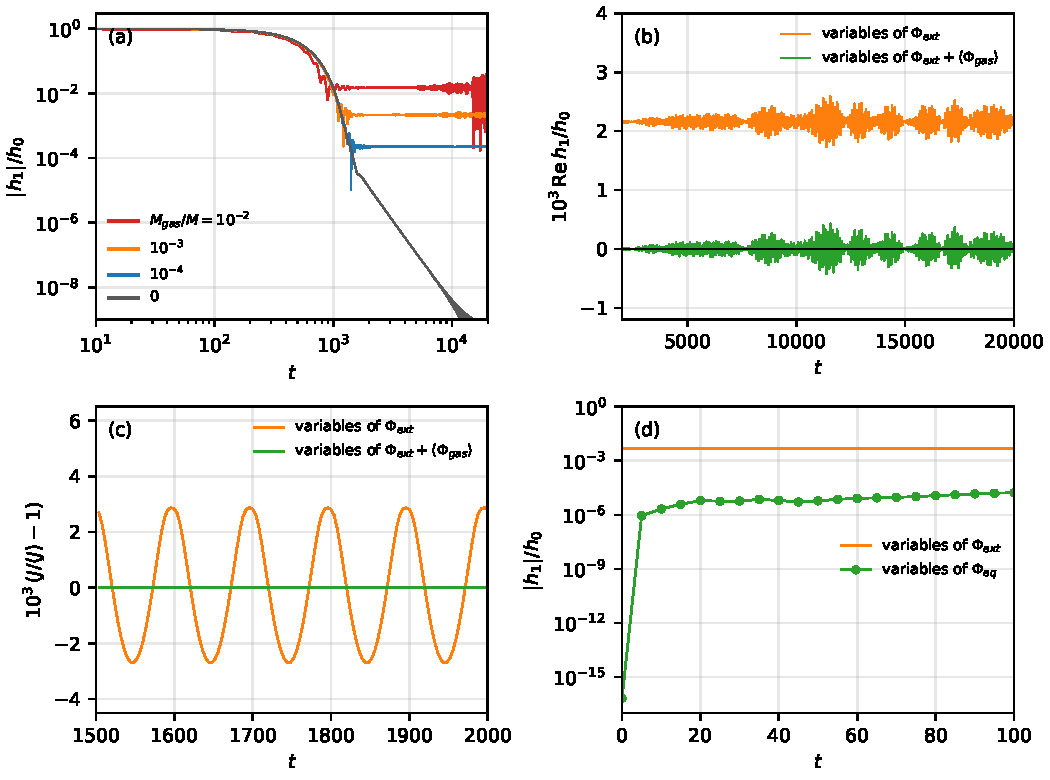
\includegraphics[width=0.85\textwidth]{figuras/validacion_mapa.pdf}}
\caption{Dependency of the function $h_1$ on the action-angle variables which are used to compute it. (a) $|h_1|/h_0$ for the mixing of the initial datum~(\ref{Eq:Pulse}) including self-gravity, computed with the action-angle variables of the external potential, for different masses of the gas. (b) Real part of $h_1/h_0$ for $M_{gas}/M = 10^{-3}$, computed with the action-angle variables of the external potential and with those of the potential $\Phi_{ext} + \langle\Phi_{gas}\rangle$, where $\langle\Phi_{gas}\rangle$ is the average of $\Phi_{gas}$ over $t\geq 2000$. (c) Relative variation of the action variable of a single computational particle for the same mass, for both sets of variables; here $\langle\Phi_{gas}\rangle$ is the average over $1500\leq t\leq 2000$, and $\langle J\rangle$ denotes the mean value over this interval. (d) $|h_1|/h_0$ for a self-consistent steady state with a distribution of angular momenta and $M_{gas}/M = 10^{-2}$, computed with the action-angle variables of the external potential and with those of $\Phi_{eq}$.}
\label{Fig:Map}
\end{figure}

Figure~\ref{Fig:Map}(a) shows the function $|h_1(t)|/h_0$ which is obtained with the action-angle variables of the external potential. When self-gravity is neglected it decays according to the law $t^{-5}$ found in the previous subsection, until it reaches the level of the numerical errors, which is of the order of $10^{-9}$, at $t\approx 10^4$. In contrast to this, when self-gravity is taken into account it settles down to a plateau: the magnitude of the time average of $h_1/h_0$ over the interval $2000\leq t\leq 2\times 10^4$ is $2.2\times 10^{-4}$, $2.2\times 10^{-3}$ and $1.5\times 10^{-2}$ for the three values of $M_{gas}/M$, whereas it is $9\times 10^{-9}$ in the absence of self-gravity. For $M_{gas}/M = 10^{-3}$ the same value, $2.16\times 10^{-3}$, is obtained with $N_J\times N_Q = 800\times 25$ and $400\times 50$. Such a plateau could be mistaken for a collective mode which is not damped.

However, the plateau disappears when the same particle data are analyzed with the action-angle variables of the potential $\Phi_{ext} + \langle\Phi_{gas}\rangle$, where $\langle\Phi_{gas}\rangle$ denotes the time average of the potential of the gas after it has become stationary. This is shown in Fig.~\ref{Fig:Map}(b) for $M_{gas}/M = 10^{-3}$: with these variables $h_1/h_0$ fluctuates about zero instead of about the value $2.16\times 10^{-3}$, and the magnitude of its time average over $2000\leq t\leq 2\times 10^4$ is reduced to $5.4\times 10^{-7}$, which is $4000$ times smaller. Therefore, the plateau is due to the choice of the coordinates and not to the dynamics. The reason is that the action variable of the external potential is not conserved along the trajectories of the gas particles in the total potential. As shown in Fig.~\ref{Fig:Map}(c), for a given particle it oscillates with the period of the radial motion; the relative difference between its largest and its smallest value is $5.6\times 10^{-3}$ for the particle shown, which has $J = 0.10$, and $4.4\times 10^{-3}$ for a particle with $J = 0.30$. In contrast to this, the action variable which belongs to the total potential is constant to within a relative variation of $2\times 10^{-5}$. Consequently, a DF which depends only on the action variable of the total potential is not independent of the angle variable of the external one, the difference between both sets of variables being of the first order in $M_{gas}/M$.

What remains after subtracting the time average is a fluctuation which is the same for both sets of variables, see Fig.~\ref{Fig:Map}(b). Its root mean square is $2.0\times 10^{-4} h_0$ in the simulation with $400\times 25$ particles, and $1.1\times 10^{-4} h_0$ and $9.6\times 10^{-5} h_0$ in those with $800\times 25$ and $400\times 50$ particles, respectively. For $M_{gas}/M = 10^{-2}$ it grows in time and is visible in Fig.~\ref{Fig:Map}(a) for $t > 10^4$; in this case its root mean square is $9.1\times 10^{-3} h_0$ with $400\times 25$ particles and $2.2\times 10^{-3} h_0$ with $800\times 25$ particles. Hence, these fluctuations are caused by the finite number of particles, which is the subject of the next subsection.

The same occurs for a self-consistent steady state. Figure~\ref{Fig:Map}(d) shows the result for the DF $\mathcal{F}_{eq}\propto J^2\exp(-J^2/\sigma_J^2)\exp[-(L - L_0)^2/\sigma_L^2]$ with $\sigma_J = 0.1$, $\sigma_L = 0.2$ and $M_{gas}/M = 10^{-2}$ in the isochrone potential, where $J$ refers to the total potential. The value of $|h_1|/h_0$ which is obtained with the action-angle variables of the external potential is $5.0\times 10^{-3}$ at all times, whereas with those of $\Phi_{eq}$ it is smaller than $10^{-16}$ at $t = 0$ and equal to $1.7\times 10^{-5}$ at $t = 100$. The small value which develops for $t > 0$ reflects the departure of the discretized steady state from stationarity, which is analyzed next.


\subsection{Stationarity of the discretized steady states}
\label{SubSec:ValStationarity}

Next, we analyze the reference simulations with $\varepsilon = 0$, in which the gas should remain in the self-consistent steady state. We consider the polytrope~(\ref{Eq:Polytrope}) with $k = 1.25$, $L_0 = 2$ and $J_{max} = 0.7$ in the Kepler potential with $M_{gas}/M = 1$, which is the largest mass ratio considered in this article and, hence, the most demanding case, and the weight function~(\ref{Eq:BDef}) with $J_1 = 0.35$ and $\sigma_1 = 0.2$. We use two quantities to measure the departure from stationarity. The first one is $|h_1^{(0)}(t)|/h_0$, which vanishes for a steady state, and the second one is the root mean square displacement of the action variables of the computational particles,
\begin{equation}
\Delta J_{rms}(t) := \left[ \frac{1}{M_{gas}}\sum\limits_{j=1}^N m_j\left( J_j(t) - J_j(0) \right)^2 \right]^{1/2},
\label{Eq:DeltaJrms}
\end{equation}
both being computed with the action-angle variables of $\Phi_{eq}$. The results for three different numbers of particles and two values of $\Delta r$ are shown in Table~\ref{Tab:Reference} and Fig.~\ref{Fig:Reference}. They reveal two different effects.

\begin{table}[htp]
\begin{center}
\begin{tabular}{lll|ccccc|ccc|c}
\hline\hline
 & & & \multicolumn{5}{c|}{$10^3\, |h_1^{(0)}|/h_0$} & \multicolumn{3}{c|}{$10^3\,\Delta J_{rms}/J_{max}$} & \\
$N_J\times N_Q$ & $\Delta r$ & $\Delta t$ & $t = 0$ & $500$ & $1000$ & $2000$ & $3900$ & $t = 1000$ & $2000$ & $4000$ & $|\Delta\mathcal{E}_{gas}/\mathcal{E}_{gas}|$ \\
\hline
$400\times 25$ & $0.1$ & $0.1$ & $1.8$ & $1.5$ & $1.5$ & $2.3$ & $10.7$ & $1.4$ & $6.3$ & $37$ & $7.7\times 10^{-6}$ \\
$400\times 25$ & $0.05$ & $0.1$ & $0.72$ & $0.44$ & $1.4$ & $2.1$ & $12.3$ & $1.7$ & $9.8$ & $42$ & $2.7\times 10^{-6}$ \\
$800\times 50$ & $0.1$ & $0.1$ & $2.0$ & $1.4$ & $1.4$ & $1.5$ & $1.7$ & $0.50$ & $0.58$ & $2.5$ & $3.0\times 10^{-6}$ \\
$1280\times 80$ & $0.1$ & $0.05$ & $2.0$ & $1.4$ & $1.4$ & $1.4$ & $1.4$ & $0.46$ & $0.41$ & $0.56$ & $1.9\times 10^{-6}$ \\
\hline\hline
\end{tabular}
\end{center}
\caption{Departure from stationarity of the reference simulations ($\varepsilon = 0$) for the polytrope with $k = 1.25$ and $M_{gas}/M = 1$ in the Kepler potential. For $|h_1^{(0)}|/h_0$ we give the largest value in the interval $[t,t+100]$. The last column is the largest relative change of the total energy up to $t = 4000$.}
\label{Tab:Reference}
\end{table}

\begin{figure}[htp]
\centerline{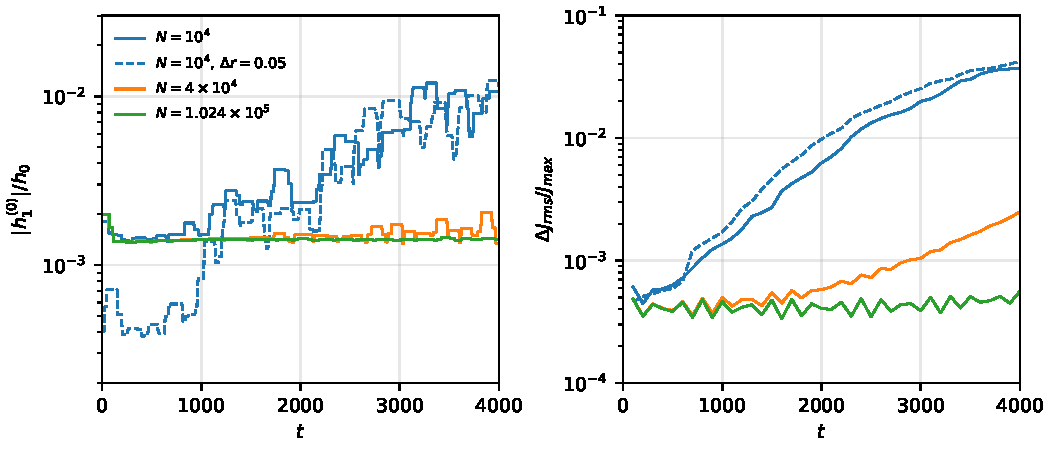
\includegraphics[width=0.85\textwidth]{figuras/validacion_referencia.pdf}}
\caption{Reference simulations ($\varepsilon = 0$) for the polytrope with $k = 1.25$ and $M_{gas}/M = 1$ in the Kepler potential, for different numbers $N = N_J N_Q$ of particles and grid spacings ($\Delta r = 0.1$ unless otherwise stated). Left panel: largest value of $|h_1^{(0)}|/h_0$ in a moving window of width $100$. Right panel: root mean square displacement~(\ref{Eq:DeltaJrms}) of the action variables of the particles.}
\label{Fig:Reference}
\end{figure}

The first effect is present from the beginning. Within the first radial periods, $|h_1^{(0)}|/h_0$ rises to a level of about $1.4$ to $2\times 10^{-3}$, which does not depend on the number of particles and is reduced by a factor between $2.5$ and $3.4$ when $\Delta r$ is halved. Its origin is the discretization error of the potential: the lattice represents a steady state of the exact potential $\Phi_{eq}$, whereas the particles move in the potential computed on the grid, which differs from $\Phi_{eq}$ by an error of the order of $\Delta r^2$. Hence, the initial configuration is slightly out of equilibrium, and the gas reacts to this. We have verified the scaling with $\Delta r$ for the Wilson model with $W_0 = 3$, $J_{max} = 0.138$ and $M_{gas}/M = 0.5$ in the isochrone potential. In this case, the root mean square over the interval $3\leq r\leq 15$ of $\delta\Phi^{(0)}$ at $t = 0$, of its time average and of the remaining oscillation, which has the frequency of the oscillating mode of this steady state, are $8.7\times 10^{-5}$, $1.7\times 10^{-4}$ and $7.7\times 10^{-5}$ in units of the largest value of $|\Phi_{gas}|$ for $\Delta r = 0.1$. They change by less than three percent when the number of particles is multiplied by four or the time step is halved, and they decrease by the factors $4.0$, $4.0$ and $3.9$ when $\Delta r$ is halved. Since this error is the same in the simulation with the perturbation and in its reference simulation, to leading order it cancels in the response~(\ref{Eq:Response}).

The second effect is a growth which sets in after a certain time. For $N = 10^4$ the quantity $|h_1^{(0)}|/h_0$ starts to grow at $t\approx 1000$ and reaches $10^{-2}$ at the end of the simulation, while the displacement of the action variables increases from $1.4\times 10^{-3} J_{max}$ at $t = 1000$ to $3.7\times 10^{-2} J_{max}$ at $t = 4000$. This growth is not reduced by halving $\Delta r$ (in fact, it becomes slightly faster), but it is delayed when the number of particles is increased: for $N = 4\times 10^4$ the displacement stays below $6\times 10^{-4} J_{max}$ up to $t = 2000$ and reaches $2.5\times 10^{-3} J_{max}$ at $t = 4000$, and for $N = 1.024\times 10^5$ both quantities remain constant up to $t = 4000$. Therefore, it is due to the discreteness of the particles, which gradually destroys the regularity of the lattice. Note that the dependency on $N$ is much stronger than the one of the fluctuations of a random sample, which are proportional to $N^{-1/2}$. The total energy is conserved to better than $10^{-5}$ in all cases; its error decreases when $\Delta r$ is reduced or $N$ is increased, but it does not depend on $\Delta t$ (see the next subsection).

For a gas of small mass the lattice is preserved over much longer times: for the polytrope with $k = 2$ and $M_{gas}/M = 0.01$ and $N = 10^4$ we find $\Delta J_{rms} = 3.6\times 10^{-5} J_{max}$ at $t = 8000$. We conclude that for $M_{gas}/M = 1$ the quiet start with $N = 10^4$ particles is reliable up to $t\approx 1000$, whereas $N\geq 4\times 10^4$ particles are required for the time span $t\leq 4000$ of our simulations.

Finally, we mention a test of the computation of the gravitational field in a situation which is dominated by self-gravity, namely the collapse of a cold homogeneous sphere of mass $M_{gas}$ and radius $R$ in the absence of an external potential. Before the shells cross each other, the shell with initial radius $r_0$ follows the cycloid $r = r_0\cos^2\theta$, $t = (\theta + \sin\theta\cos\theta)/\sqrt{2GM_{gas}/R^3}$. For $\Delta r = 0.01 R$, the median of the relative error of the radii of the shells with $0.1 < r_0/R < 0.9$ at the time $t = 0.8\sqrt{R^3/(GM_{gas})}$ is $1.8\times 10^{-5}$ for $N = 200$ and $4.3\times 10^{-6}$ for $N = 400$ shells, which corresponds to second-order convergence in $1/N$.


\subsection{Time step, amplitude of the perturbation and comparison with the linearized equations}
\label{SubSec:ValResponse}

We now turn to the response~(\ref{Eq:Response}) of the gas to a perturbation of the form~(\ref{Eq:InitialData}). We first analyze its dependency on the time step. To this purpose we consider the polytrope with $k = 1$ and $M_{gas}/M = 1$ in the Kepler potential (with the remaining parameters as in the previous subsection), $\varepsilon = 0.1$, $N_J\times N_Q = 400\times 25$ and $\Delta r = 0.1$, and we repeat the simulation and its reference simulation with $\Delta t = 0.2$, $0.1$ and $0.05$. Figure~\ref{Fig:TimeStep} shows the difference between the responses $\delta\Phi_{res}$ which are obtained with different time steps, measured with the norm~(\ref{Eq:deltaPhiNorm}) for $r_a = 3$ and $r_b = 7.5$. In the intervals $0\leq t\leq 250$, $250\leq t\leq 500$, $500\leq t\leq 750$ and $750\leq t\leq 1000$, the difference between the results for $\Delta t = 0.1$ and $\Delta t = 0.05$, relative to the largest value of $\|\delta\Phi_{res}\|$ in the respective interval, is at most $6.6\times 10^{-4}$, $3.0\times 10^{-3}$, $5.6\times 10^{-3}$ and $1.9\times 10^{-2}$, and the one between $\Delta t = 0.2$ and $\Delta t = 0.05$ is larger by the factors $4.4$, $5.0$, $6.4$ and $6.3$. For a second-order method one expects the factor five, and for a fourth-order one the factor $17$. The same conclusion is obtained from the simulation with $\varepsilon = 0.1$ alone, for which we have a further run with $\Delta t = 0.025$: relative to the latter, the error of the potential for $\Delta t = 0.05$ is smaller than the one for $\Delta t = 0.1$ by the factors $4.7$, $4.1$, $3.9$ and $3.4$ in the same intervals, where again the factor five is expected for a second-order method. Hence, in the presence of self-gravity the time integration is only second-order accurate, in contrast to the fourth-order convergence found in section~\ref{SubSec:ValFree}. This reduction of the order is to be expected, since the field which results from the linear weights~(\ref{Eq:Deposit}) is continuous but not differentiable with respect to the positions of the particles, whereas the fourth-order accuracy of the composition method requires a smooth force.

\begin{figure}[htp]
\centerline{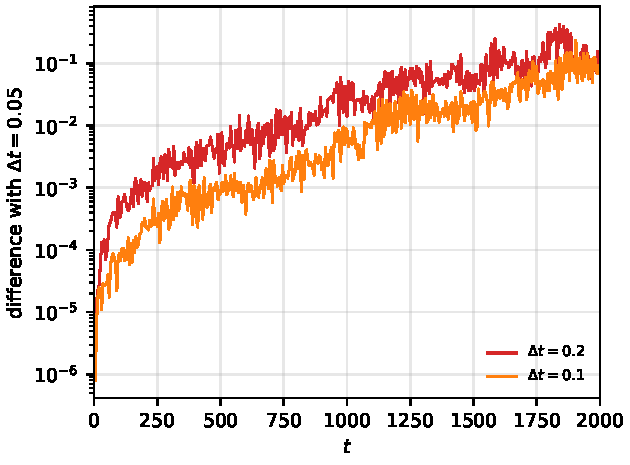
\includegraphics[width=0.5\textwidth]{figuras/validacion_paso.pdf}}
\caption{Dependency of the response on the time step for the polytrope with $k = 1$ and $M_{gas}/M = 1$ in the Kepler potential, with $\varepsilon = 0.1$ and $N = 10^4$. Shown is the norm~(\ref{Eq:deltaPhiNorm}) of the difference between the response $\delta\Phi_{res}$ obtained with the indicated time step and the one obtained with $\Delta t = 0.05$, divided by the largest value of $\|\delta\Phi_{res}\|$.}
\label{Fig:TimeStep}
\end{figure}

The error due to the time step grows with time. For $\Delta t = 0.1$ it amounts to two percent of the response at $t = 1000$. At later times the differences between the three simulations grow to several ten percent. However, this is not a consequence of the time integration: at $t = 2000$ the radii of corresponding particles in the simulations with $\Delta t = 0.1$ and $\Delta t = 0.025$ differ by up to $3.3$, which shows that for $N = 10^4$ the trajectories of the individual particles are no longer correlated, in accordance with the loss of the quiet start at $t\approx 1000$ found in the previous subsection. In contrast to this, the frequency of the oscillation of $\delta\Phi_{res}$, determined from its periodogram over $500\leq t\leq 2000$, is $0.14770$ for the three time steps, and the relative error of the total energy, $1.8\times 10^{-5}$, is the same for $\Delta t = 0.2$, $0.1$, $0.05$ and $0.025$, such that it is not due to the time integration.

Next, we compare the response with the solution of the linearized equations obtained with the method of section~\ref{SubSec:LinSolver}. For a gas of small mass we consider the polytropes with $k = 0.75$, $1$, $1.5$ and $2$ and $M_{gas}/M = 0.01$ in the Kepler potential, with $N_J\times N_Q = 400\times 25$, $\Delta r = 0.1$ and $\Delta t = 0.1$. In these cases the response decays algebraically (see section~\ref{Sec:FixedL}): at $t = 1000$ the magnitude of $\chi_1$ has decreased to a fraction between $2.6\times 10^{-3}$ (for $k = 0.75$) and $1.8\times 10^{-4}$ (for $k = 2$) of its initial value. With $\varepsilon = 0.1$, the difference between the function $\chi_1(t)$ obtained from the PIC code and the one obtained from the linearized equations is smaller than $1.2\times 10^{-4}|\chi_1(0)|$ for all $0\leq t\leq 2000$ and the four values of $k$. Relative to the largest value of $|\chi_1|$ in the respective interval, it is at most $1.2\times 10^{-4}$ for $0\leq t\leq 500$ and between $0.3$ and $0.5$ percent for $500\leq t\leq 1000$. With $\varepsilon = 0.5$ the corresponding numbers are $5\times 10^{-4}$ and $1.4$ percent. Therefore, for this mass ratio the two methods, which are based on entirely different discretizations, agree with each other to better than one percent while the response decays by more than two orders of magnitude, and the dependency on the amplitude of the perturbation is weak.

For $M_{gas}/M = 1$ the situation is different, since the response depends on $\varepsilon$ even for rather small amplitudes. We consider again the polytrope with $k = 1.25$, for which the linearized equations predict an oscillating mode (see section~\ref{Sec:FixedL}), and compare three simulations with $\varepsilon = 0.1$, $0.03$ and $0.01$ which share the lattice with $N_J\times N_Q = 1280\times 80$ points, the time step $\Delta t = 0.05$ and the reference simulation, such that they only differ from each other in the amplitude. In order to compare two oscillating signals we use the quantity
\begin{equation}
\kappa(t_0) := \frac{\sum_j w(t_j - t_0)\,\chi_1(t_j)\,\chi_1^{lin}(t_j)^*}{\sum_j w(t_j - t_0)\,|\chi_1^{lin}(t_j)|^2},\qquad
w(\tau) := \cos^2\left( \frac{\pi\tau}{T_w} \right)\quad\hbox{for $|\tau|\leq \frac{T_w}{2}$},
\label{Eq:kappa}
\end{equation}
and $w(\tau) := 0$ otherwise, where $\chi_1^{lin}$ refers to the solution of the linearized equations, the sums extend over the output times $t_j$ which are common to both solutions, and $T_w = 200$, which corresponds to about five periods of the oscillation. The magnitude of $\kappa(t_0)$ is the ratio between the amplitudes of the two signals in the window centered at $t_0$, and its phase is their phase difference, such that $-d\arg\kappa/dt_0$ is the difference between their frequencies. Since $\kappa$ depends linearly on $\chi_1$, it can be extrapolated to $\varepsilon = 0$.

\begin{table}[htp]
\begin{center}
\begin{tabular}{l|cccccc}
\hline\hline
$\varepsilon$ & $t_0 = 500$ & $1000$ & $1500$ & $2000$ & $2500$ & $3000$ \\
\hline
$0.1$ & $0.869$ & $0.614$ & $0.591$ & $0.762$ & $0.913$ & $0.830$ \\
$0.03$ & $0.976$ & $0.946$ & $0.923$ & $0.908$ & $0.924$ & $0.906$ \\
$0.01$ & $0.992$ & $0.990$ & $0.986$ & $0.978$ & $1.004$ & $0.997$ \\
\hline
$0$ (linear) & $1.000$ & $1.013$ & $1.020$ & $1.017$ & $1.048$ & $1.048$ \\
$0$ (quadratic) & $0.997$ & $1.004$ & $1.017$ & $1.024$ & $1.064$ & $1.063$ \\
\hline\hline
\end{tabular}
\end{center}
\caption{The ratio $|\kappa(t_0)|$ between the amplitudes of the response obtained from the PIC code and from the linearized equations, see Eq.~(\ref{Eq:kappa}), for the polytrope with $k = 1.25$ and $M_{gas}/M = 1$ in the Kepler potential and three amplitudes of the perturbation ($N = 1.024\times 10^5$, $\Delta t = 0.05$). The last two rows refer to the extrapolation to $\varepsilon = 0$ by means of a straight line through the results for $\varepsilon = 0.01$ and $0.03$ and of a parabola through the three results, respectively.}
\label{Tab:Amplitude}
\end{table}

The results are shown in Table~\ref{Tab:Amplitude}. For $\varepsilon = 0.1$ the amplitude of the response falls to $56$ percent of the one predicted by the linearized equations at $t_0 = 1300$, and for $\varepsilon = 0.03$ to $91$ percent at $t_0 = 2000$, whereas for $\varepsilon = 0.01$ it stays between $0.977$ and $1.005$ of the latter for $t_0\leq 2000$ and between $0.95$ and $1.06$ up to $t_0 = 3900$. The simulation with $\varepsilon = 0.1$, $N = 10^4$ and $\Delta t = 0.1$ gives $|\kappa| = 0.871$ and $0.629$ at $t_0 = 500$ and $1000$, such that for as long as its quiet start lasts it agrees with the one with $N = 1.024\times 10^5$ to within two percent. Hence, the loss of amplitude is not a numerical artifact but a nonlinear effect; its origin is discussed in section~\ref{Sec:FixedL}. Extrapolating the three results to $\varepsilon = 0$ we obtain an amplitude which lies between $1.00$ and $1.05$ times the linear one for $t_0\leq 2000$ when a straight line through the two smallest amplitudes is used, and between $0.99$ and $1.06$ when a parabola through the three amplitudes is used. For $250\leq t_0\leq 2000$ the phase of $\kappa$ grows linearly with $t_0$, at the rate $1.3\times 10^{-4}$ for $\varepsilon = 0.03$ and $5.8\times 10^{-5}$ for $\varepsilon = 0.01$, which means that the frequency of the oscillation decreases slightly with the amplitude. For the extrapolation to $\varepsilon = 0$ the rate is $2.5\times 10^{-5}$ (straight line) and $0.7\times 10^{-5}$ (parabola), which is of the order of the accuracy with which the frequency of the linearized solution is known (see the next subsection). Finally, for $\varepsilon = 0.01$ the fluctuations of $\kappa$ between consecutive windows are of the order of one percent for $t_0\leq 2000$ and of four percent afterwards. Note that for this amplitude the function $h_1^{(0)}/\varepsilon$ of the reference simulation is $2.5$ times larger than the response itself, such that the latter is obtained as the difference of two much larger quantities.

We conclude that for $M_{gas}/M = 1$ the PIC code reproduces the solution of the linearized equations within a few percent, provided that $N\approx 10^5$ particles and amplitudes $\varepsilon\leq 0.01$ are used. \EJ{For $k = 0.75$, $1$ and $2$ the simulations of section~\ref{Sec:FixedL} with $M_{gas}/M = 1$ still have $N = 10^4$ particles and $\varepsilon = 0.1$. The ones with $N = 1.024\times 10^5$, $\Delta t = 0.05$ and $\varepsilon = 0.03$ and $0.1$ have been run on the cluster and their analysis is pending; the default parameters quoted at the end of section~\ref{SubSec:PIC} have to be adapted accordingly.}


\subsection{Linearized equations and gain of the self-consistent loop}
\label{SubSec:ValLinear}

In order to estimate the accuracy of the solutions of the linearized equations, we have repeated the computation for the polytrope with $k = 1.25$ and $M_{gas}/M = 1$ of the previous subsection with half the time step, with twice the number of points in $Q$ and with twice the number of rows in $J$, and compared the results with the one for the default values $N_J\times N_Q = 1600\times 32$ and $\Delta t = 0.5$ by means of the quantity~(\ref{Eq:kappa}) in the interval $300\leq t_0\leq 3900$. Halving $\Delta t$ changes the amplitude of $\chi_1$ by $0.2$ percent and its frequency by $-0.9\times 10^{-5}$, doubling $N_Q$ changes them by $-0.3$ percent and $1.4\times 10^{-5}$, and doubling $N_J$ by $0.01$ percent and $0.7\times 10^{-6}$, respectively. Since the differences in the frequency accumulate in the phase, the difference between the functions $\chi_1(t)$ themselves grows linearly in time; at $t = 4000$ it reaches $3.5$, $5.9$ and $0.3$ percent of the amplitude in the three cases.

An independent test is provided by the gain $\lambda(\omega)$, which is computed by a completely different method (see section~\ref{SubSec:GainNum}). For the polytropes with $k = 0.75$, $1$ and $1.25$ and $M_{gas}/M = 1$ in the Kepler potential, the solution of the linearized equations settles down to an oscillation whose frequency, determined with the method of section~\ref{SubSec:Fits} in the window $300\leq t\leq 1500$, is $0.14169$, $0.14783$ and $0.15330$, respectively, whereas the equation $\lambda(\omega_d) = 1$ yields $\omega_d = 0.14169$, $0.14785$ and $0.15326$. Hence, both methods agree to within $4\times 10^{-5}$.

Finally, the method for the computation of the gain for a distribution of angular momenta, which differs from the one for the reduced model in the integration of the orbits, in the quadrature nodes and in the radial grid, should reproduce the results for the reduced model when the distribution in $L$ is narrow. We have verified this for DFs of the form $\mathcal{F}_{eq} = \alpha(E_0 - E)^k g(L)$, where $g$ is a Gaussian function centered at $L_0$ whose width is equal to $10^{-3} L_0$, using the total potential $\Phi_{eq}$ of the corresponding polytrope~(\ref{Eq:Polytrope}) of the reduced model. For $k = 2$ and $M_{gas}/M = 1$ we obtain $\lambda = 0.497963$ and $0.674389$ at $\omega = 0.5\,\Omega_{min}$ and $0.9\,\Omega_{min}$, against $0.497970$ and $0.674400$ for the reduced model. For $k = 3$ and $M_{gas}/M = 1$, and for $k = 2$ and $M_{gas}/M = 0.1$, the values of $\lambda$ at $\omega = 0.5\,\Omega_{min}$ and at the edge of the band agree to within $4\times 10^{-6}$. At the edge of the band for $k = 2$ and $M_{gas}/M = 1$ the difference is $1.8\times 10^{-4}$ ($0.820117$ against $0.819933$), because for a distribution of finite width the edge of the frequency band is slightly displaced.
